\chapter{Diskussion}

In diesem Kapitel werden die Ergebnisse dieser Arbeit diskutiert, als erstes wird sich mit den PSI \& PHI Winkeln auseinander gesetzt und anschließend werden die Ergebnisse, der \ac{SNP}s in den \ac{EP}s, erörtert.


\section{Ramachandran Diskussion}

Wie in Kapitel \ref{sec:ramachandran} gezeigt, ist der Ramachandran Plot geeignet, um zu überprüfen, ob und wie sich die Winkel bei einem \ac{SNP} im Protein verändern. Dabei war die Idee zu schauen ob an einem \ac{SNP} Winkel auftreten, welche für die Proteine einer speziellen Proteinfamilie sehr unwahrscheinlich sind. Denn es wird erwartet, dass Proteine in einer Proteinfamilie eine gewisse strukturelle Ähnlichkeit besitzen, wie in Kapitel \ref{sec:pfam} beschrieben. 

Doch leider hat sich gezeigt, dass sich die Mutation nicht aufgrund der Winkelveränderung bestimmen lässt. Denn z.B. \ac{Abb} \ref{fig:ramachandran_PF01287} betrachtet wird, sieht man dass die Winkel am \ac{SNP} immer noch

Generell hat sich gezeigt, dass in einer Proteinfamilie nicht nur spezifische PSI und PHI Winkel auftreten, sondern fast alle Winkel im Spektrum des Möglichen. Wenn wir beispielsweise \ac{Abb} \ref{fig:ramachandran_PF00883} ansehen, so fällt auf, dass fast der gesamte Plot blau ist. Denn jeder blaue Punkt steht für eine PSI/PHI Winkel Kombination, welche in dieser \ac{Pfam} vorkommt. 

\begin{figure}
    \centering
    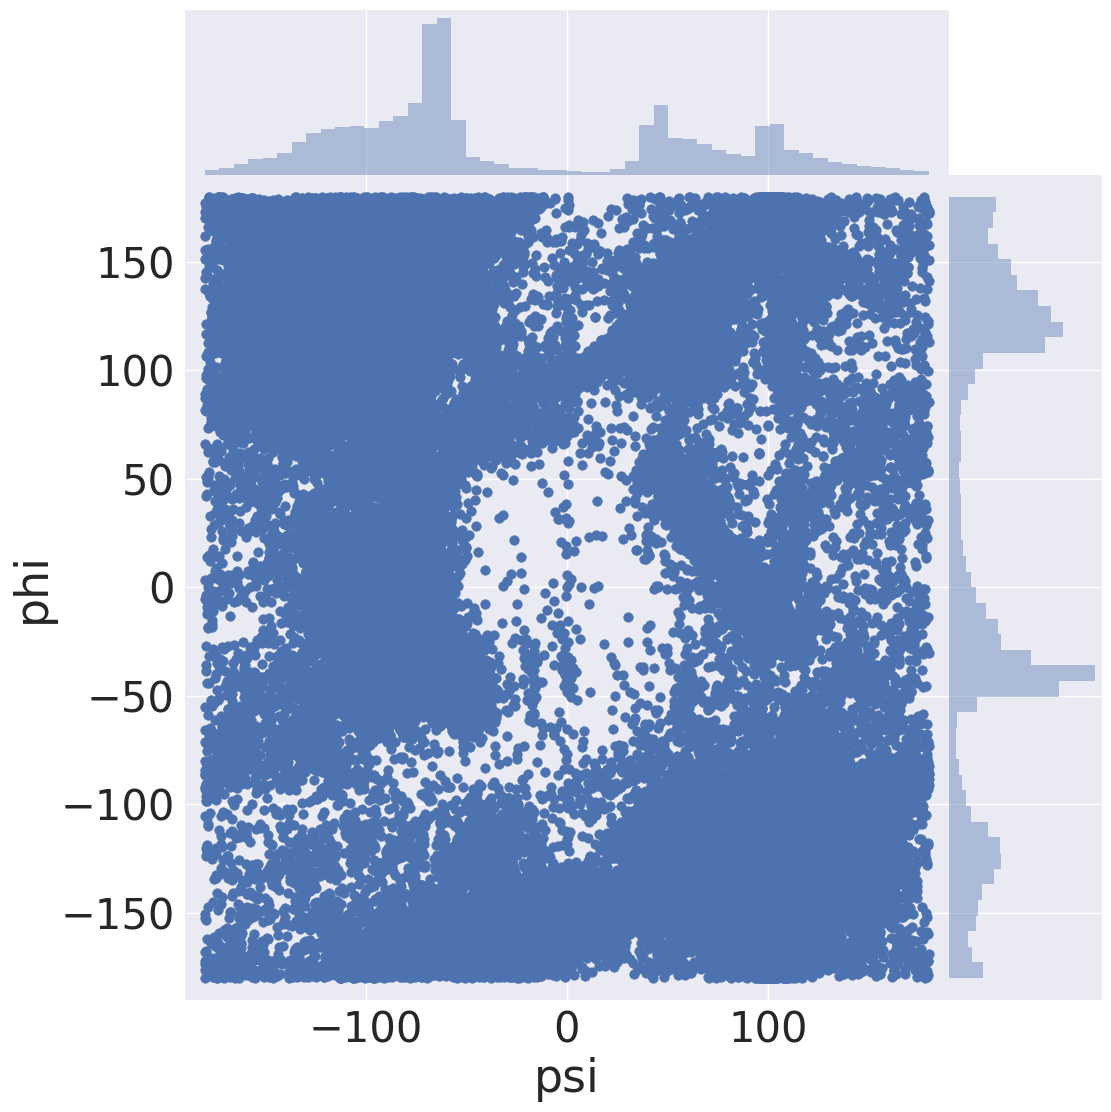
\includegraphics[width=.90\textwidth]{images/ramachandranplot_PF00883.png}
    \caption{Ramachandran Plot der Pfam \texttt{PF00883}, exakter Aufbau wie \ac{Abb} \ref{fig:ramachandran_PF01287}.}
    \label{fig:ramachandran_PF00883}
\end{figure}

Es ist noch wichtig zu erwähnen, dass dieser Ansatz sehr allgemein war, es wäre noch möglich gewesen die exakte Domäne des Proteins herauszusuchen, in der jeweilige \ac{SNP} liegt und in der \ac{Pfam} auch nur diese Sequenz zu berücksichtigen. Oder eine \emph{Kernel Density Estimation}\cite{Parzen.1962} vorzunehmen, um so die relative Verteilung der Winkel zu analysieren. Da dieser Ansatz jedoch nicht sehr viel versprechend aussah, wurde er nicht weiter verfolgt, damit so mehr Zeit für die Analyse der \ac{EP}s zu Verfügung steht.

Mit den bisherigen Erkenntnissen, lässt sich abschließend festhalten, dass es nicht möglich ist, auf Grundlage der PSI \& PHI Winkel Veränderung, einen \ac{SNP} zu klassifizieren.


\section{SNPs in Energieprofilen}
\label{sec:snps_in_eps}
In Kapitel \ref{chap:ergebnisse} wurden die Ergebnisse dieser Arbeit vorgestellt. Dort ist zu sehen, dass \ac{SNP}s \ac{EP}s verändern können. Nun soll diskutiert werden, ob sich \ac{SNP}s mittels \ac{EP}s annotieren lassen können.

\subsection{Energieniveau Veränderung}

Jede Aminosäure hat ein spezielles Spektrum an Energiewerten, welche sie annehmen kann. Die Idee war nun zu überprüfen, ob die ausgetauschte Aminosäure am \ac{SNP} einen Energiewert annimmt, welcher sehr unwahrscheinlich für sie ist.

Betrachten wir die Energiespektren der Aminosäuren in \ac{Abb} \ref{fig:energy_ranges} und die Veränderung der Energie in \ac{Abb} \ref{fig:comp_plot_MSH2}. So sehen wir, dass im Protein \texttt{MSH2} Glycin gegen Tryptophan ausgetauscht wurde. Das zu erwartende Spektrum für Glycin reicht von -29,7 bis 2,2. Somit liegt der Tryptophan \ac{SNP} mit dem Energiewert -30,5 außerhalb des Spektrums. Doch mit der neuen Aminosäure, muss auch das neue Spektrum berücksichtigt werden, in diesem Fall, dass von Tryptophan, welches von -38,8 bis -4,2 reicht. Somit liegt der Wert -30,5 im 1. Quartil, sodass der Energiewert am \ac{SNP} im normalen Spektrum liegt, in welchem Tryptophan zu erwarten ist.

Als weiteres Beispiel dient die \ac{Abb} \ref{fig:comp_plot_ACADM}, hier wurde im Protein \texttt{ACADM} Isoleuchin, an Position 78, gegen Threonin ausgetauscht. Isoleucin hatte an dieser Position einen Energiewert von -33,4, Threonin hingegen hat einen Energiewert von -14,8. Das zu erwartende Spektrum für Threonin reicht von -32,7 bis 1,3. Somit liegt der Energiewert am \ac{SNP} im 1. Quartil von Threonin, also auch hier keine Auffälligkeiten zu beobachten.

Damit steht fest, die Veränderungen des Energieniveaus kann nicht auf Grundlage des Spektrums, der jeweiligen Aminosäure, klassifiziert werden. Da keine Ausreißer außerhalb der zu erwartenden Energiewerte gefunden wurden. 


\subsection{Energiewert Veränderung am SNP}

\begin{figure}
    \centering
    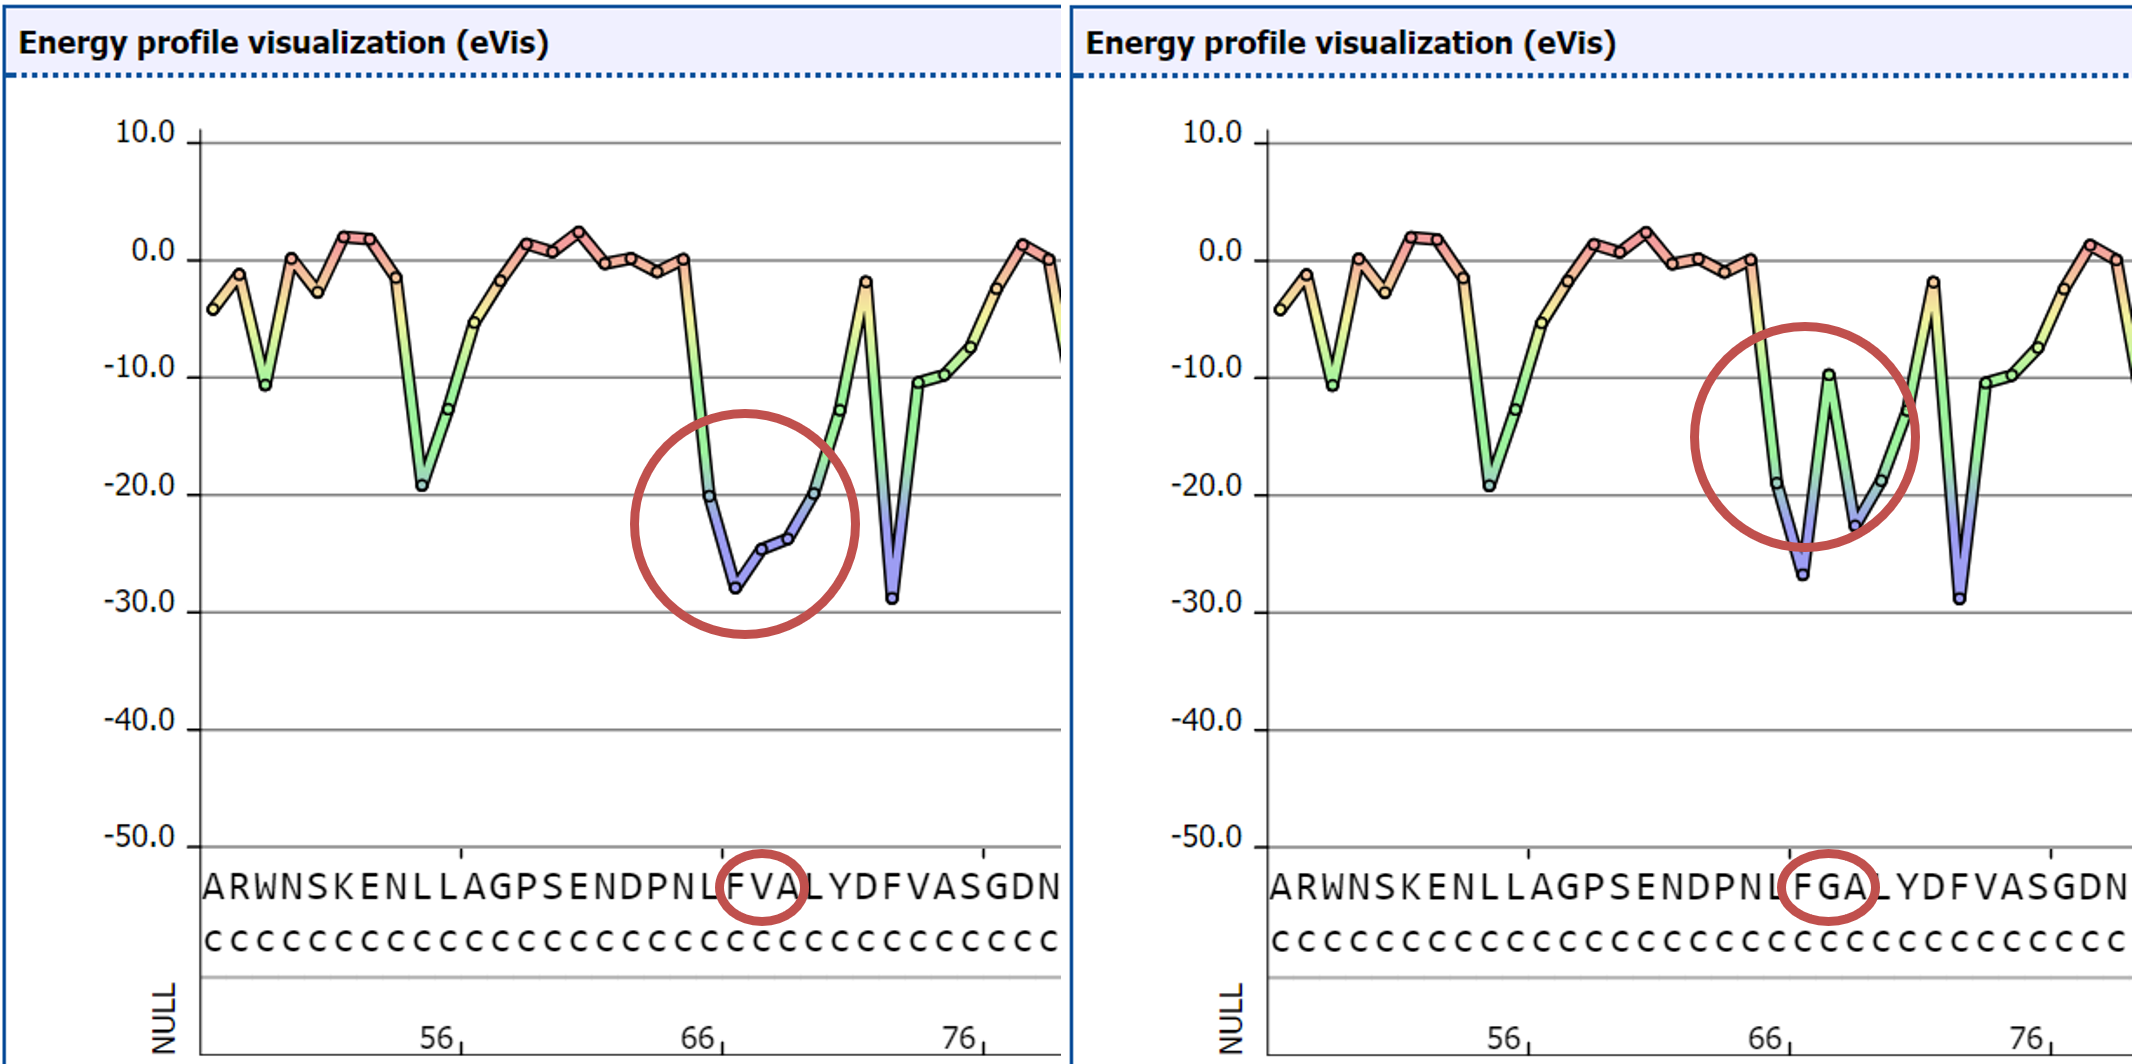
\includegraphics[width=.99\textwidth]{images/ep_vs_snp.png}
    \caption{\ac{eVis} Darstellung vom ePros Webserver (Kapitel \ref{sec:epros}) eines Ausschnittes eines \ac{EP}s. Die original Sequenz befindet sich links und die Sequenz mit dem \ac{SNP}(rote Markierung) ist rechts. Auf der Abszisse sind die Aminosäuren im Einbuchstabencode aufgetragen, siehe Tabelle \ref{tab:amino_table}. Darunter ist die Sekundärstruktur als Buchstabencode aufgetragen. Unten ist die Aminosäureposition in 10er Schritten aufgetragen. Auf der Ordinate befinden sich die Energiewerte.}
    \label{fig:ep_vs_snp}
\end{figure}

Bei dem Vergleich in Kapitel \ref{sec:snps_in_eps} von \ac{EP}s mit \ac{SNP}s gegen unmutierte \ac{EP}s, ist aufgefallen, dass sich die \ac{EP}s signifikant an den \ac{SNP} Positionen unterscheiden. Zum Verständnis ist ein \ac{EP} (mit und ohne \ac{SNP}) in \ac{Abb} \ref{fig:ep_vs_snp} dargestellt. In der \ac{Abb} ist eine 2D-Visualisierung eines \ac{EP}s gezeigt. Auf der Abszisse sind die Aminosäuren im Einbuchstabencode aufgetragen, während auf der Ordinate die Energiewerte eingetragen sind. Die beiden Darstellungen unterscheiden sich nur durch die Substitution von Valin durch Glycin, so ist hier deutlich die Energiewert Differenz zwischen den beiden Darstellungen zu erkennen. So besitzt im Protein Valin an der Position 68 einen Energiewert von -25. Der Glycin \ac{SNP} hingegen, besitzt einen Energiewert von -10, so ergibt sich eine Delta von 15. Valin ist eine hydrophobe Aminosäure, während Glycin eine hydrophile Aminosäure ist, von daher ist es nicht überraschend, dass sich auch die Energiewerte des Proteins an dieser Stelle bei einem Austausch verändern. Dies zeigt uns deutlich, dass wir drastische Veränderungen der Proteinstruktur auch in den \ac{EP}s sehen.

Sieht man sich nun mit diesem Wissen \ac{Abb} \ref{fig:comp_plot_MSH2} an, so fällt auf, dass der gutartige \ac{SNP} das \ac{EP} von \texttt{MSH2}, fast gar nicht verändert. Dies wird auch durch die chemischen Eigenschaften von Valin bestätigt, denn Valin ist unpolar, genauso wie Isoleucin, welches es ersetzt hat. Zudem haben beide Aminosäuren in etwa die gleiche Größe. Generell lässt sich sagen, dass das \ac{EP} sich fast gar nicht verändert und die gesamte Energiedifferenz bei gerade mal -0,006 liegt. Dies passt alles sehr gut zu der ClinVar Annotation, welche sagt, dass dieser \ac{SNP} gutartig ist.

Betrachten wir nun die untere \ac{Abb} in \ref{fig:comp_plot_MSH2}, so sehen wir, dass sich die Energie stark am \ac{SNP} verändert. Nämlich von -17,1 auf -30,4, dies ist ein Delta von 13,3. Generell wurde auch gezeigt, dass sich die Energie im gesamten Protein viel stärker, als im gutartigen \ac{SNP}, in der oberen \ac{Abb} verändert. Wenn die chemischen Eigenschaften von Glycin begutachtet werden, fällt auf, dass es polar ist. Bei Tryptophan hingegen handelt es sich um eine unpolare Aminosäure. Zusätzlich ist Glycin die kleinste Aminosäure, während Tryptophan wesentlich größer ist. Auch dies passt gut zur ClinVar Annotation, welche besagt, dass es sich hierbei um ein pathogenes \ac{SNP} handelt.

Sehr ähnlich verhält es sich mit der \ac{Abb} \ref{fig:comp_plot_ACADM}, im oberen Bild ist ein gutartiges \ac{SNP} des Gens \texttt{ACADM} dargestellt. Hier ist wie in \ac{Abb} \ref{fig:comp_plot_MSH2} nur eine kleine Veränderung der Energie zu sehen. Bei Methionin handelt es sich um eine hydrophobe Aminosäure, genau wie bei Isoleucin. So scheint dieser \ac{SNP} chemisch keine große Veränderung zu verursachen. Diese Annahme wird auch von der ClinVar Annotation gutartig bestätigt. 

Wird hingegen das untere Bild der \ac{Abb} \ref{fig:comp_plot_ACADM} angesehen, so fällt eine sehr starke Veränderung des Energieniveaus, um 18,6 am \ac{SNP}, auf. Nach bisherigem Wissen würden wir diesen \ac{SNP} also als pathogen einordnen, dies ist richtig, wenn die ClinVar Annotation hinzugezogen wird. Auch die chemischen Eigenschaften der Threonin unterscheiden sich von den der Aminosäure Isoleucin, denn Threonin ist polar und Isoleucin nicht. 

Somit lässt sich abschließend sagen, dass auf Grundlage des Deltas, zwischen dem \ac{EP} mit und ohne \ac{SNP}, es möglich ist ein \ac{SNP} zu klassifizieren, da pathogene Mutationen immer ein größeres Delta aufweisen, als gutartige.


\section{Anwendbarkeit der EPs zur Annotation von SNPs im Panel}

In Kapitel \ref{sec:snps_in_eps} wurde gezeigt, dass pathogene \ac{SNP}s die Energie deutlich stärker verändern, als Gutartige.  Die Auswertung der \ac{SNP}s aus Tabelle \ref{tab:snps_memb} und \ref{tab:snps_glob} ergab, dass dies möglich ist und ein MCC von 0,8 für globuläre und sogar 1,0 für Membran assoziierte Proteine erreicht werden kann, wie in Kapitel \ref{sec:snp_auswertung} zu sehen ist. Doch jetzt stellt sich die Frage, ob die Erkenntnisse der Arbeit genutzt werden können, um die, im Illumina TruSight Myeloid Sequencing Panel auftretenden Gene, zu annotieren. 

Dafür wurde zuerst per Hand versucht, die einzelnen Gensequenzen herunterzuladen und anschließend in Swissmodel zu modellieren. Doch leider lieferte dies nicht die gewünschten Ergebnisse, denn die Coverage war in den meisten Fällen sehr schlecht. So bewegte sich z.B. die Coverage für \texttt{NRAS} zwischen 1-4\%, sodass nur einzelne Helices abgedeckt waren. Es wurden noch vier andere Gene aus dem Panel getestet, aber auch diese hatten keine allzu große Coverage, zusätzlich war der Vorgang sehr zeitaufwendig. 

\begin{table}[H]
    \centering
    \caption{Illumina TruSight Myeloid Sequencing Panel Gene \emph{coverage}, Transkriptlänge ist mit UTRs und CDS angegeben.}
    \label{tab:illumina_coverage}
    \resizebox{\linewidth}{!}{%
    \begin{tabular}{lllll}
    \hline
    \multicolumn{1}{|l|}{Genname} & \multicolumn{1}{l|}{Genlänge (bp)} & \multicolumn{1}{l|}{Transkriptlänge} & \multicolumn{1}{l|}{PDB-ENSP} & \multicolumn{1}{l|}{PDB Coverage} \\ \hline
    IDH1 & 29847 & 2298 & 1t09.A & 17,97\% \\
    KDM6A & 239425 & 5438 & 3avr.A & 9,58\% \\
    JAK2 & 143793 & 5285 & 4z32.A & 9,18\% \\
    NRAS & 12425 & 4449 & 3con.A & 3,84\% \\
    RAD21 & 28931 & 3749 & 4pju.B & 3,71\% \\
    NOTCH1 & 51418 & 9371 & 3eto.A & 3,06\% \\
    \end{tabular}}
\end{table}

Aus diesem Grund wurde der EnsemblBioMart\footnote{\url{https://www.ensembl.org/biomart}} hinzugezogen, dieser ermöglicht es dem Nutzer leicht, spezielle Datensätze mit verschiedensten Filtern herunterzuladen. So wurde in diesem Fall die Genliste des Illumina Panels mit 54 Genen im BioMart eingefügt und Genlänge, Transkriptlänge, korrespondierende \ac{PDB} Einträge und deren Start und Stopp Position abgefragt, dargestellt in Tabelle \ref{tab:illumina_coverage}. Die Start und Stopp Position der \ac{PDB} Einträge wurde mit der Transkriptlänge verrechnet, sodass eine prozentuale Coverage abgebildet werden kann. Wie zu sehen ist, besitzt \texttt{IDH1} die beste Coverage mit 17,97\%. Dies ist leider viel zu wenig, um eine erfolgreiche Berechnung eines \ac{EP}s durchzuführen. Die zweitbeste Coverage hatte \texttt{KDM6a} mit 9,58\%, was nochmal deutlich weniger ist als die vorherige Coverage.

An dieser Stelle sei gesagt, die minimale Coverage und Sequenzidentität für eine erfolgreiche Annotation, ist in Kapitel \ref{sec:min_coverage} diskutiert. 

Bei den anderen Genen des Panels sah es leider noch schlechter aus, denn von den 54 Genen insgesamt, weisen gerade mal 6 Gene überhaupt eine Teilabdeckung auf.

\begin{table}[]
    \centering
    \caption{VariantPlex Solid Tumor Kit Coverage, Transkriptlänge ist mit UTRs und CDS angegeben.}
    \label{tab:variantplex_coverage}
    \resizebox{\linewidth}{!}{%
    \begin{tabular}{lllll}
    \hline
    \multicolumn{1}{|l|}{Genname} & \multicolumn{1}{l|}{Genlänge (bp)} & \multicolumn{1}{l|}{Transkriptlänge} & \multicolumn{1}{l|}{PDB-ENSP} & \multicolumn{1}{l|}{Coverage} \\ \hline
    ATM & 146618 & 12954 & 5np0.A & 23,58\% \\
    IDH1 & 29847 & 2298 & 1t09.A & 17,97\% \\
    H3F3A & 10150 & 799 & 3av2.A & 16,90\% \\
    RB1 & 178235 & 4840 & 4elj.A & 15,17\% \\
    BRAF & 205437 & 2480 & 4mnf.A & 12,26\% \\
    PIK3CA & 91979 & 9093 & 2rd0.A & 11,73\% \\
    SMO & 24673 & 3738 & 5v56.A & 10,27\% \\
    RHOA & 53853 & 2031 & 1ftn.A & 9,45\% \\
    JAK2 & 143793 & 5285 & 4z32.A & 9,18\% \\
    CCND1 & 13387 & 4307 & 2w96.A & 6,27\% \\
    ALK & 728792 & 6220 & 4fob.A & 5,66\% \\
    DDR2 & 156027 & 3096 & 2wuh.A & 5,43\% \\
    ROS1 & 137555 & 7435 & 3zbf.A & 4,01\% \\
    SMAD4 & 56651 & 8495 & 1dd1.A & 3,14\% \\
    NOTCH1 & 51418 & 9371 & 3eto.A & 3,06\% \\
    MYCN & 6443 & 2602 & 5g1x.B & 2,34\%
    \end{tabular}}
\end{table}

Um zu überprüfen, ob es sich bei dem Illumina Panel nicht um eine unglückliche Ausnahme handelt, wurde noch ein zweites Panel überprüft. Das \emph{VariantPlex Solid Tumor Kit}\footnote{\url{http://archerdx.com/variantplex/solid-tumor}} umfasst 67 Gene im Zusammenhang mit soliden Tumoren. Doch auch hier ist nur ein Bruchteil der Gene (16) aufgeklärt und von diesen 16 Genen, ist keines komplett strukturell aufgeklärt, siehe Tabelle \ref{tab:variantplex_coverage}. Die höchste Coverage hat \texttt{ATM} mit 23,58\%. Dies ist jedoch immer noch zu wenig um damit eine Homologie Modellierung durchzuführen. Auch dieses Panel beinhaltet \texttt{IDH1} und weist damit ebenfalls eine Coverage von 17,97\% auf, gefolgt von \texttt{H3F3A} mit einer Coverage von 16,90\%. Bei den restlichen Treffern fällt die Coverage stark ab und 51 Gene haben sogar gar keine.

Somit lässt sich abschließend sagen, dass sich \ac{APs} (noch) nicht für die Annotation von \ac{SNP}s im Illumina TruSight Myeloid Sequencing Panel eignen, da einfach noch zu wenige Strukturen aufgeklärt sind. Denn ohne aufgeklärte Struktur macht es keinen Sinn, ein Homologie Modellierung durchzuführen, denn wie in \ref{sec:min_coverage} gezeigt, würde das Ergebnis unbrauchbar sein. Sodass keine \ac{EP} Berechnung möglich ist. 


\subsection{Minimale Coverage und Sequenzidentität}
\label{sec:min_coverage}

In diesem Abschnitt wird diskutiert, welche minimale Coverage ein Protein haben muss, damit es Sinn macht ein \ac{EP} dafür zu berechnen. Denn es hat sich herausgestellt, dass die Vorhersage eines \ac{SNP}s sehr stark abhängig von dem verwendeten Template ist.

\begin{figure}[H]
    \centering
    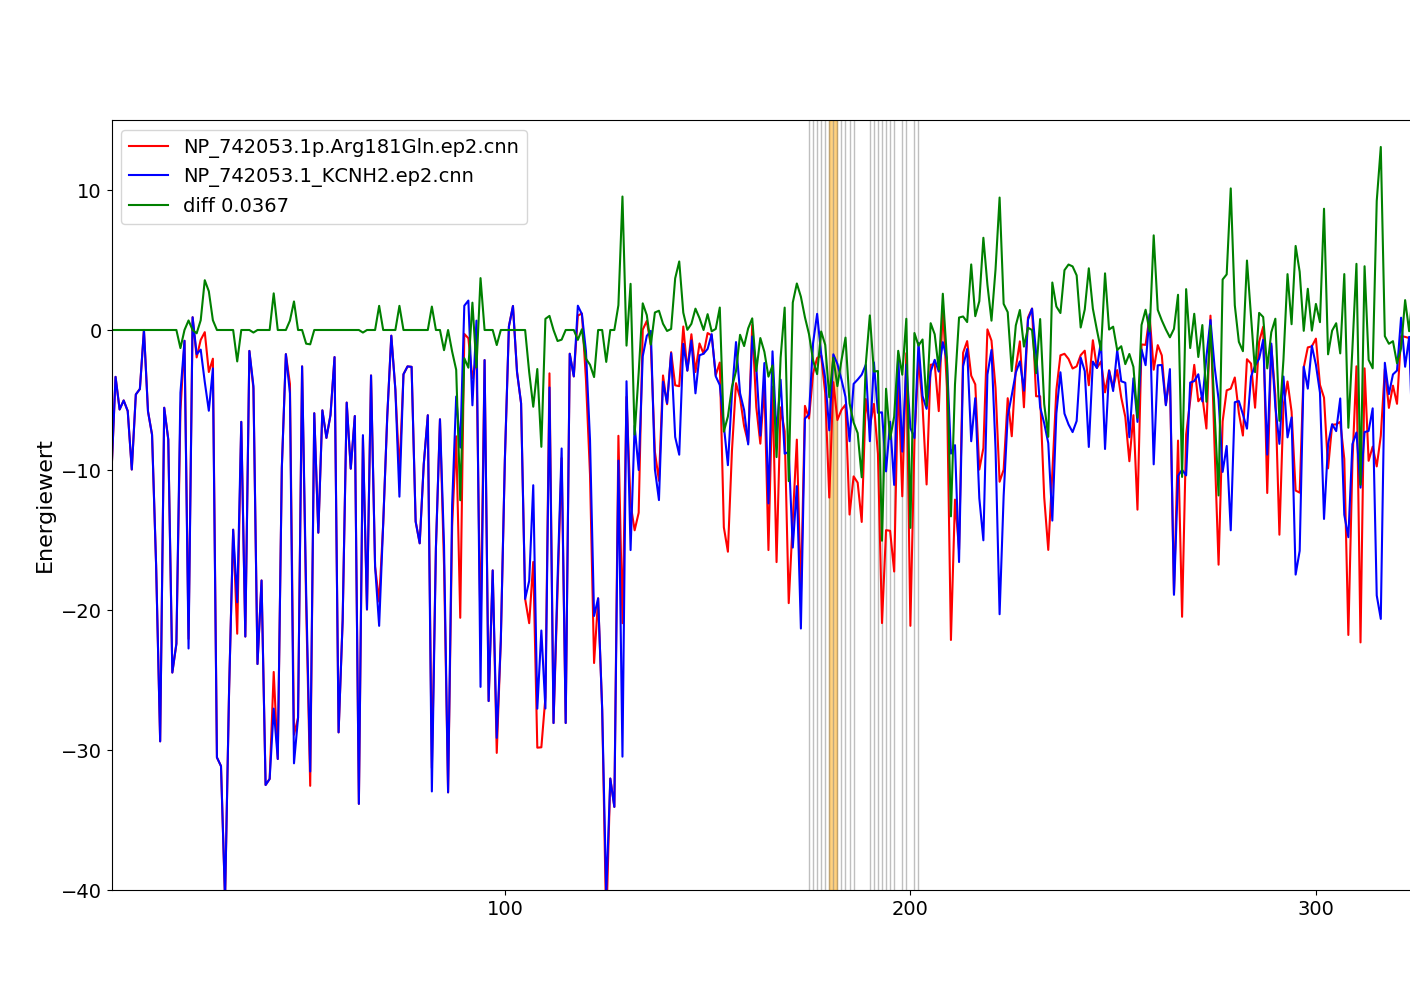
\includegraphics[width=.99\textwidth]{images/comp_plot_KCNH2_Arg181Gln.png}
    \caption{Ausschnitt aus dem Protein \texttt{KCNH2} mit gutartigem \ac{SNP} an Position 181. Der Plot ist exakt wie \ref{fig:comp_plot_MSH2} aufgebaut.}
    \label{fig:fail_ep}
\end{figure}

In \ac{Abb} \ref{fig:fail_ep} ist ein gutartiger \ac{SNP} im Protein \texttt{KCNH2} dargestellt. Mit den bisherigen Erkenntnissen würden wir kaum eine Veränderung von der Referenz zum \ac{SNP} \ac{EP} erwarten. Doch wie zu sehen ist, ist eine sehr starke Differenz zwischen den beiden \ac{EP}s vorhanden. 

Wenn wir nun Tabelle \ref{tab:multiple_subs_snps} betrachten sehen wir, dass \texttt{KCNH2} im Vergleich zum Template 74,20\% Coverage aufweist, mit einer Sequenzidentität von 96,5\%. Hierbei scheint bereits die um 1\% schlechtere Sequenzidentität, im Vergleich zu \texttt{SDHB}, dafür zu sorgen, dass die Modellierung sehr schlecht wird. Dies zeigt sich auch am QMEAN Wert von -5,38. Also können wir festhalten, dass die Sequenzidentität sehr wichtig ist für eine erfolgreiche Homologie Modellierung, die Empfehlung dieser Arbeit ist >97\%.

Die Coverage ist ebenfalls wichtig, denn wenn nur ein Teil der Proteinstruktur aufgeklärt ist, so können mögliche Nachbarn bei der \ac{EP} Berechnung nicht berücksichtigt werden. Doch sie ist nicht so essentiell wie die Sequenzidentität, denn z.B. das Gen \texttt{MUTHY} hat nur eine Coverage von 51,4\%, siehe Tabelle \ref{tab:multiple_subs_snps}, aber dennoch einen QMEAN von -1,8. Also kann festgehalten werden, dass es keine klare Grenze für die Coverage gibt, es jedoch sinnvoll ist, die größtmögliche Coverage anzustreben, da sonst Interaktionen mit fehlenden Bereichen nicht berücksichtigt werden können.

% nochmal einen MUTYH SNP checken



\section{Problem mit dem Datensatz}
\label{sec:probleme_mit_dem_datensatz}

In diesem Abschnitt werden die Probleme mit dem Datensatz aus \ref{sec:snp_analyse} diskutiert, mit dem Fokus auf die korrekte Trennung der \ac{SNP}s.

Wie in Tabelle \ref{tab:mcc_table} zu sehen ist, wurde im besten Fall nur ein MCC von 0,8 erreicht. Dafür mussten allerdings drei \ac{SNP}


Dies könnte z.B. daran liegen, dass die Datengrundlage, also die ClinVar Variationen nicht alle richtig annotiert sind. Als Beispiel dienen die \ac{SNP}s Asp167His und Ala272Val, in der Tabelle \ref{tab:multiple_subs_snps}. So sind diese \ac{SNP}s zwar als gutartig eingestuft, doch mir ist bei der Auswahl ein Fehler unterlaufen, denn diese \ac{SNP}s haben auch pathogene Annotationen auf der ClinVar. Aus diesem Grund wurden anschließend nochmals alle \ac{SNP}s überprüft und die \ac{SNP}s mit Widersprüchen nicht für die MCC Berechnung berücksichtigt.

In einem weiteren Versuch den Datensatz zu erweitern, wurden noch \ac{SNP}s, welche nur von einem Autor eingetragen wurden, angeschaut. Doch hier zeigte sich, dass die Daten nicht verlässlich genug sind. Denn in Tabelle \ref{tab:multiple_subs_snps} ist ein gutartiges \ac{SNP} mit nur einem Autoren zu sehen, welches nach dem hier diskutiertem Ansatz eigentlich als pathogen annotiert werden müsste. So können wir nicht sagen, ob der Autor recht hat und unsere Vorhersage falsch ist, oder umgekehrt.

Auf der einen Seite gab es viele Proteine mit vollständig aufgeklärter Struktur, wie \texttt{ABCG2}\footnote{\url{http://www.rcsb.org/pdb/explore/explore.do?structureId=5NJ3}} oder \texttt{KCNH2}\footnote{\url{http://www.rcsb.org/pdb/explore/explore.do?structureId=5VA1}}, doch leider hatten diese keine mehrfach bestätigten \ac{SNP}s in der ClinVar Datenbank. 
Auf der anderen Seite gab es schon Gene mit vielen mehrfach bestätigen \ac{SNP}s, jedoch gab es keine vollständige 3D-Struktur zu den Genen, wie z.B. \texttt{BRCA1} und \texttt{BRCA2}.

Dazu kam noch die Tatsache, dass bei Genen, welche nicht zu 100\% aufgeklärt waren, viele \ac{SNP}s außerhalb der bekannten Struktur lagen, dies war z.B. bei \texttt{PMS2} der Fall war. Bei diesem Gen war, zum Zeitpunkt dieser Arbeit, 39\% der Struktur aufgeklärt. Nur leider konnten von den 19 gutartigen \ac{SNP}s aus der ClinVar nur 2 in die Datenbank einfließen, da die restlichen nicht auf der aufgeklärten Struktur gelegen haben.

Ein weiteres Problem war, dass \ac{SNP}s auf verschiedenen Transkripten gelegen haben. So war z.B. das Template des Gens \texttt{MLH1} von einem Transkript signifikant schlechter, als das Andere. Wobei hier zu sagen ist, dass die oben genannten Gründe einen deutlich größeren Einfluss haben.



\section{Zu wenige Daten}

Es wäre es sehr wünschenswert wenn mehr Patienten Daten zu Verfügung stehen würden, so könnte eine einfache Datenbank aller bekannten Patienten \ac{SNP}s schon hilfreich sein, um zu verstehen, ob verschiedene \ac{SNP}s öfter in speziellen Leukämien auftreten.

Zudem haben wir keine Informationen über Alter, Geschlecht oder Ähnliches, weder in den SNP Daten der ClinVar, noch in den Illumina Daten aus dem Panel, sodass wir auch hier nichts extra berücksichtigen können. Was aber hilfreich sein könnte, da z.B. wie auf \ac{Abb} \ref{fig:Age_AML_ALL} zu sehen ist eine \ac{ALL} hauptsächlich im Kindesalter auftritt.

Bedauerlich, da, wie in Abb. 1.2 zu sehen ist, eine ALL hauptsächlich im Kindesalter auftritt und somit Altersangaben bzgl. der Patientenproben wichtig wären, um die richtigen Diagnosen ??? zu stellen / Schlüsse zu ziehen 

\textbf{hier muss noch was kommen, also das Kapitel ist nicht rund}

